\section{Differential branching ratio extraction}
\label{sec:Lb_BRsummary}

In this chapter differential branching ratio values for the $\Lb\to\Lz\mumu$ decay are calculated 
relative to the \Lb\ra\jpsi\Lz branching ratio as a function of \qsq.
These values are directly obtained from the fit to the rare sample by parameterising
the downstream and long yields with the following formula:
%
\begin{equation}
N(\Lz\mumu)_{k}  = \left[ \frac{\mathrm{d}\mathcal{B}(\Lz\mumu)/\mathrm{d}\qsq}{\mathcal{B}(\jpsi\Lz)} \right]  \cdot
N(\jpsi\Lz)_{k} \cdot \epsilon^{\mathrm{rel}}_{k} \cdot \frac {\Delta\qsq} { \mathcal{B}(\jpsi\to\mumu) },
\label{eq:ield_from_BR}
\end{equation}
\noindent
where $k = $(LL,DD), $\Delta\qsq$ is width of the \qsq bin and the only free paramater is the relative
branching fraction ratio.% over the \jpsi channel.
%To move from relative differential rate to absolute one, we again multiply by the $\Lb\to\jpsi\Lz$ branching fraction.
For the \jpsi\to\mumu branching ratio the value reported in the PDG book,
$\mathcal{B}(\jpsi\to\mumu) = (5.93 \pm 0.06)\cdot 10^{-2}$~\cite{PDG2014}, is used.
%
Tab.~\ref{tab:Lb_effSummary} summarises the total relative efficiencies for downstream and long candidates
together with their correlated and uncorrelated errors, where the correlation is intended between the downstream and long 
samples. %In the table is reported the absolute value of the total relative efficiency and the absolute value of the
%uncorrelated error.
On the table the uncorrelated error corresponds to the total systematic error on the efficiency.
The correlated error is given in per cent form since it can be applied to either downstream, long candidates or their combination.
This includes the PDF systematic described in Sec.~\ref{sec:Lb_yield_sys} and the systematic due to the uncertainty on \jpsi\to\mumu branching ratio.

\begin{table}
\centering
\caption{Absolute values of the total relative efficiency and the absolute value of the 
uncorrelated error, together with relative values of correlated error. }
\begin{tabular}{lccccc} \hline\hline
\qsq interval [\gevgevcccc] 	 & Eff. (DD) 	 &  $\sigma_{uncorr}^{DD}$	 & Eff. (LL) 	 & $\sigma_{uncorr}^{LL}$ 	 & Correlated err. \\
\hline

0.1--2.0    &  0.694  &  0.058  &  1.136  &  0.066  &  1.012\%    \\
2.0--4.0    &  0.693  &  0.027  &  0.907  &  0.047  &  2.697\%    \\
4.0--6.0    &  0.699  &  0.018  &  0.964  &  0.044  &  2.697\%    \\
6.0--8.0    &  0.733  &  0.020  &  0.953  &  0.048  &  2.697\%    \\

11.0--12.5  &  1.254  &  0.032  &  1.140  &  0.057  &  3.356\%    \\
15.0--16.0  &  1.260  &  0.035  &  1.035  &  0.060  &  2.977\%    \\
16.0--18.0  &  1.163  &  0.029  &  0.997  &  0.048  &  1.727\%    \\
18.0--20.0  &  1.023  &  0.027  &  0.782  &  0.040  &  2.697\%    \\
\hline
1.1--6.0    &  0.696  &  0.032  &  0.950  &  0.058  &  1.012\%    \\
15.0--20.0  &  1.132  &  0.014  &  0.927  &  0.031  &  1.423\%    \\
\hline
\end{tabular}
\label{tab:Lb_effSummary}
\end{table}

In Fig. \ref{fig:corrDDLLplots}, the branching ratio obtained by fitting the downstream and long samples independently.

\begin{figure}
\centering
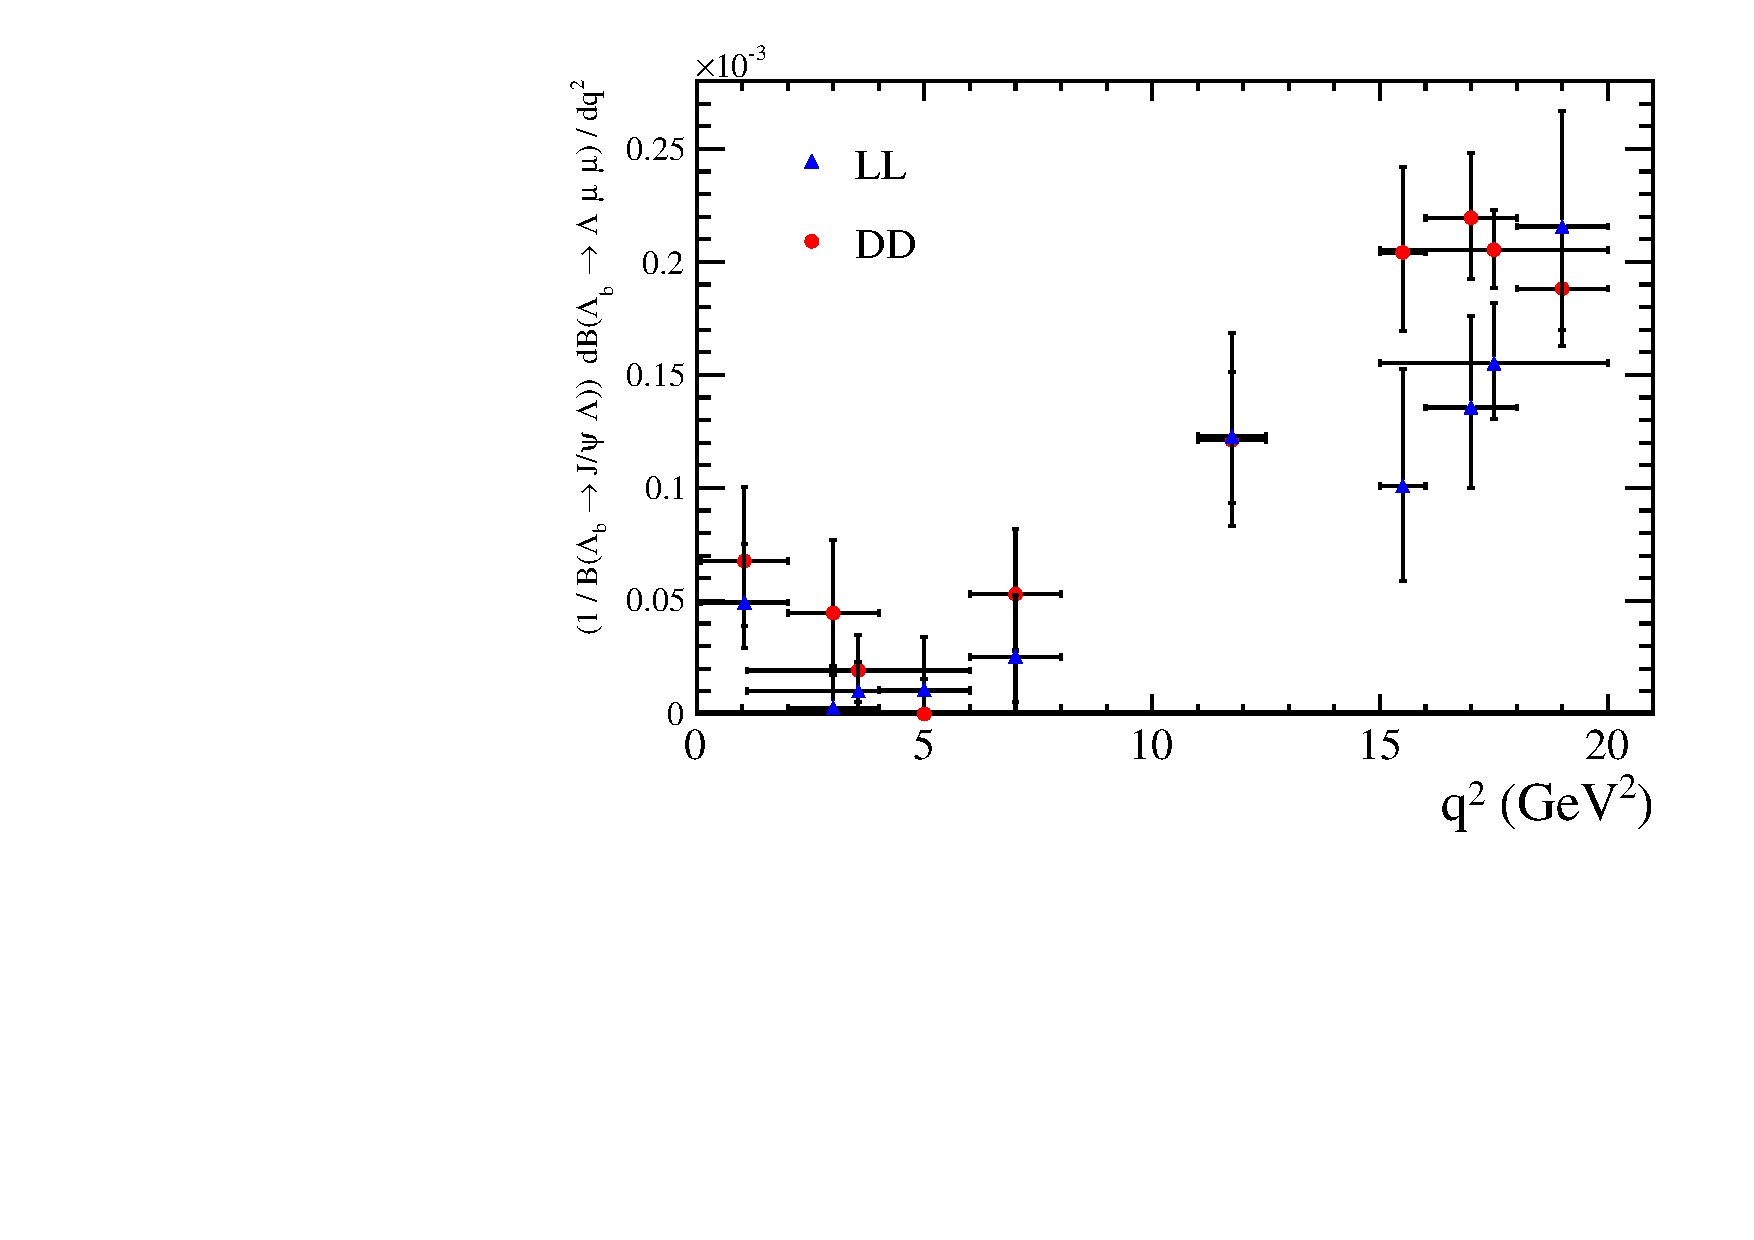
\includegraphics[width=0.8\textwidth]{Lmumu/figs/q2result_both.pdf}
\caption{Measured values of \Lb\ra\Lz\mumu relative to the \Lb\to\jpsi\Lz decay as a function of \qsq bins
obtained fitting the downstream and long samples independently.
Errors shown represent statistical and systematic uncertainties.}
\label{fig:corrDDLLplots}
\end{figure}

%We performed $\chi^2$ consistency test to verify consistency between DD and LL results. We evaluate $\chi^2$ as

%\begin{equation}
%\chi^2 = \sum \frac{(Y(DD)_i - Y(LL)_i)^2}{(\sigma_{uncorr}^{LL})^2_i + (\sigma_{uncorr}^{DD})^2_i}
%\end{equation}

%where $Y(DD)_i$ and $Y(LL)_i$ are corrected yields for DD and LL events in each bin and $\sigma_{uncorr}^{LL}$($\sigma_{uncorr}^{DD}$) their uncorrelated error,
%including statistical on rare and normalisation channels and uncorrelated systematic error. 
%The result is a $\chi^2$ of 7.0 with 4 degrees of freedom corresponding to a p-value of 0.14.


%\begin{table}
%\centering
%\renewcommand{\arraystretch}{1.3}
%\begin{tabular}{lc} \hline\hline
%\qsq bin 	 &  $\mathrm{d}\mathcal{B}(\Lz\mumu)/\mathrm{d}\qsq / \mathcal{B}(\jpsi\Lz)$ ($10^{-3}$)\\
%\hline
%\multicolumn{2}{c}{Down-down events} \\ \hline 
%\hline

%0.1-2.0  & $    0.0676^{+0.0323}_{-0.0279} \text{(stat)} ^{+0.0055}_{-0.0064} \text{(sys)} ^{+0.0008}_{-0.0008} \text{(norm)} $ \\
%2.0-4.0  & $    0.0447^{+0.0324}_{-0.0275} \text{(stat)} ^{+0.0021}_{-0.0022} \text{(sys)} ^{+0.0005}_{-0.0006} \text{(norm)} $ \\
%4.0-6.0  & $    0.0000^{+0.0155}_{0.0000} \text{(stat)} ^{+0.0000}_{-0.0000} \text{(sys)} ^{+0.0000}_{-0.0000} \text{(norm)} $ \\
%6.0-8.0  & $    0.0530^{+0.0287}_{-0.0248} \text{(stat)} ^{+0.0020}_{-0.0021} \text{(sys)} ^{+0.0007}_{-0.0007} \text{(norm)} $ \\
%11.0-12.5  & $    0.1211^{+0.0300}_{-0.0273} \text{(stat)} ^{+0.0049}_{-0.0053} \text{(sys)} ^{+0.0010}_{-0.0014} \text{(norm)} $ \\
%15.0-16.0  & $    0.2042^{+0.0369}_{-0.0338} \text{(stat)} ^{+0.0082}_{-0.0084} \text{(sys)} ^{+0.0022}_{-0.0022} \text{(norm)} $ \\
%16.0-18.0  & $    0.2196^{+0.0276}_{-0.0260} \text{(stat)} ^{+0.0066}_{-0.0068} \text{(sys)} ^{+0.0023}_{-0.0024} \text{(norm)} $ \\
%18.0-20.0  & $    0.1882^{+0.0259}_{-0.0241} \text{(stat)} ^{+0.0070}_{-0.0071} \text{(sys)} ^{+0.0020}_{-0.0020} \text{(norm)} $ \\

%\hline
%1.1-6.0  & $    0.0192^{+0.0157}_{-0.0138} \text{(stat)} ^{+0.0010}_{-0.0011} \text{(sys)} ^{+0.0002}_{-0.0002} \text{(norm)} $ \\
%15.0-20.0  & $    0.2054^{+0.0168}_{-0.0161} \text{(stat)} ^{+0.0039}_{-0.0040} \text{(sys)} ^{+0.0022}_{-0.0022} \text{(norm)} $ \\

%\hline
%\multicolumn{2}{c}{Long-long events} \\ \hline
%\hline
%0.1-2.0  & $    0.0493^{+0.0258}_{-0.0200} \text{(stat)} ^{+0.0030}_{-0.0033} \text{(sys)} ^{+0.0009}_{-0.0010} \text{(norm)} $ \\
%2.0-4.0  & $    0.0027^{+0.0186}_{0.0000} \text{(stat)} ^{+0.0002}_{-0.0002} \text{(sys)} ^{+0.0001}_{-0.0001} \text{(norm)} $ \\
%4.0-6.0  & $    0.0107^{+0.0234}_{0.0000} \text{(stat)} ^{+0.0005}_{-0.0006} \text{(sys)} ^{+0.0002}_{-0.0002} \text{(norm)} $ \\
%6.0-8.0  & $    0.0253^{+0.0271}_{-0.0198} \text{(stat)} ^{+0.0014}_{-0.0015} \text{(sys)} ^{+0.0005}_{-0.0005} \text{(norm)} $ \\

%11.0-12.5  & $    0.1228^{+0.0451}_{-0.0391} \text{(stat)} ^{+0.0071}_{-0.0076} \text{(sys)} ^{+0.0020}_{-0.0020} \text{(norm)} $ \\
%15.0-16.0  & $    0.1009^{+0.0513}_{-0.0413} \text{(stat)} ^{+0.0063}_{-0.0069} \text{(sys)} ^{+0.0016}_{-0.0017} \text{(norm)} $ \\
%16.0-18.0  & $    0.1356^{+0.0397}_{-0.0348} \text{(stat)} ^{+0.0066}_{-0.0072} \text{(sys)} ^{+0.0022}_{-0.0022} \text{(norm)} $ \\
%18.0-20.0  & $    0.2157^{+0.0497}_{-0.0438} \text{(stat)} ^{+0.0120}_{-0.0129} \text{(sys)} ^{+0.0035}_{-0.0035} \text{(norm)} $ \\
%\hline
%1.1-6.0  & $    0.0101^{+0.0127}_{-0.0099} \text{(stat)} ^{+0.0006}_{-0.0007} \text{(sys)} ^{+0.0002}_{-0.0002} \text{(norm)} $ \\
%15.0-20.0  & $    0.1551^{+0.0260}_{-0.0239} \text{(stat)} ^{+0.0055}_{-0.0058} \text{(sys)} ^{+0.0025}_{-0.0026} \text{(norm)} $ \\
%\hline
%\end{tabular}
%\caption{Values of corrected relative branching fraction for DD and LL events with statistical, correlated and uncorrelated error shown separately. }
%\label{tab:corrDDLL}
%\end{table}

%Finally, we combine DD and LL results by a weighted average of the two using the uncorrelated errors as weight, $w_i = 1/(\sigma_i^{uncorr})^2$.
%Using weighted average for each bin the combined result is

%\begin{equation}
%y_{combined} = \sum {w_i \cdot Y_i} / \sum {w_i}
%\end{equation}

%and its error

%\begin{equation}
%\sigma_{combined} = \sqrt{1 / \sum { \sigma_i^{-2} }}.
%\end{equation}

%The correlated error is then calculated on the combined yield using the relative values in table \ref{tab:effSummary}.

The combined result, obtained fitting both samples simoultaneouly is shown in Fig.~\ref{fig:Lb_combBR}.
Values are also reported are reported in Tab.~\ref{tab:Lb_combBR}, where the statistical
error on the rare channel (stat) and the total systematic error (stat) are shown separately.
The statistical error is calculated using the MINOS tool, which returns an asymmetric interval.
The normalisation and systematic errors are evaluated by pushing the efficiencies and normalisation yields
up and down by the value of their errors are re-performing the fit. %DD and LL errors are different so each one is taken in accout properly.
The different efficiencies used have an effect on the branching ratio and the full difference with respect to the default 
fit is taken as systematic uncertainty in each direction.


 \begin{figure}[tbph]
 \centering
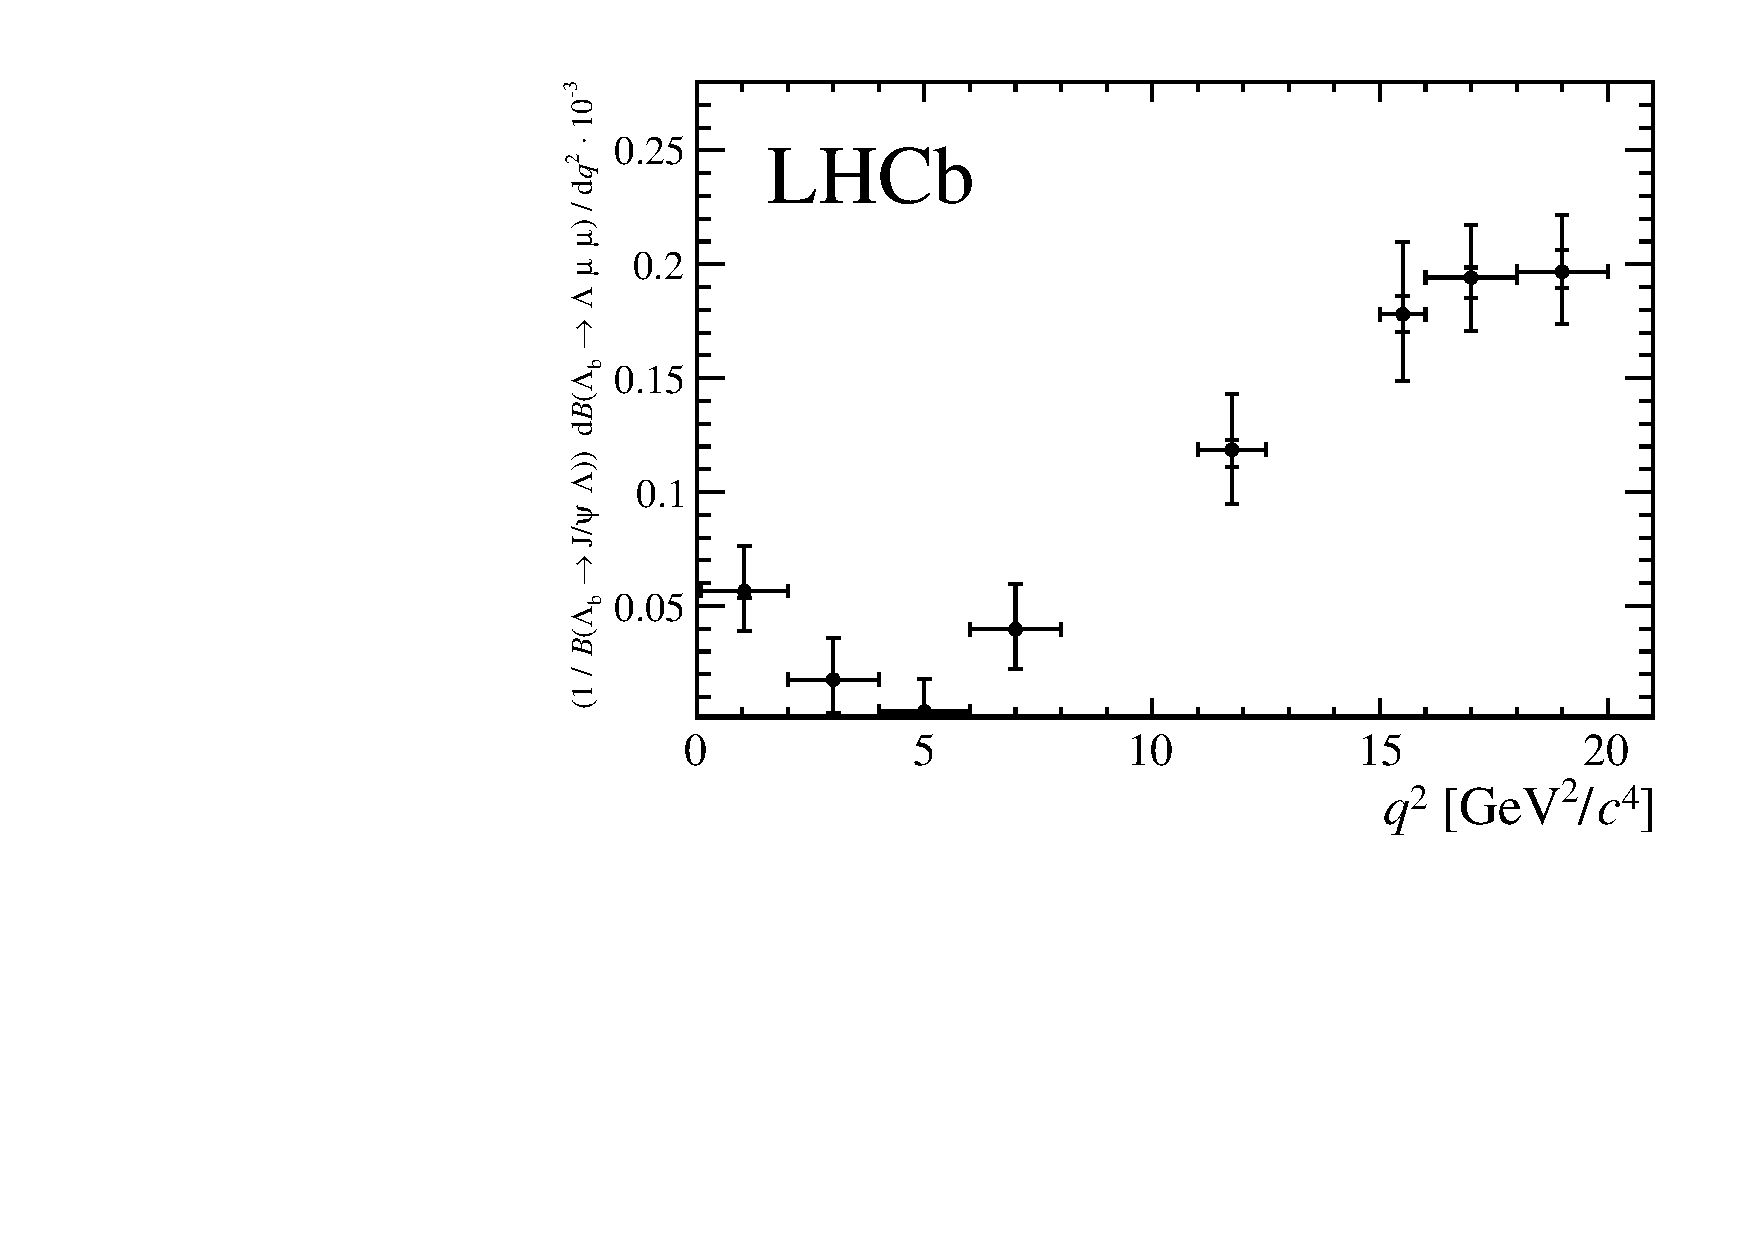
\includegraphics[width=0.8\textwidth]{Lmumu/figs/combined_result_2err.pdf}
\caption{Branching fraction of the \decay{\Lb}{\Lz\mumu} decay
  normalised to the \decay{\Lb}{\jpsi\Lz} mode. The inner error
  represents the systematic error and the outer error the total
  error.} 
   \protect\label{fig:Lb_combBR}
 \end{figure}

\begin{table}
\centering
\renewcommand{\arraystretch}{1.2}
\caption{Differential branching fraction of the \decay{\Lb}{\Lz\mumu}
  decay relative to \decay{\Lb}{\jpsi\Lz} decays,
 where the uncertainties are statistical and systematic, respectively.}
\begin{tabular}{cccccc}
  \qsq interval  [\gevgevcccc] & &\multicolumn{4}{c}{ $\frac{\deriv\BF(\decay{\Lb}{\Lz\mumu})/\deriv\qsq}{\BF(\decay{\Lb}{\jpsi\Lz})} \cdot 10^{-3} [(\gevgevcccc)^{-1}]$} \\
\hline
0.1 -- 2.0   & &0.56 & $^{+0.20}_{-0.17}$ & $^{+0.03}_{-0.03}$ & \\
2.0 -- 4.0   & &0.18 & $^{+0.18}_{-0.15}$ & $^{+0.01}_{-0.01}$ & \\
4.0 -- 6.0   & &0.04 & $^{+0.14}_{-0.04}$ & $^{+0.01}_{-0.01}$ & \\
6.0 -- 8.0   & &0.40 & $^{+0.20}_{-0.17}$ & $^{+0.01}_{-0.02}$ &\\
                                                 
11.0 -- 12.5 & &1.19 & $^{+0.24}_{-0.23}$ & $^{+0.04}_{-0.07}$& \\
15.0 -- 16.0 & &1.78 & $^{+0.31}_{-0.28}$ & $^{+0.08}_{-0.08}$&\\
16.0 -- 18.0 & &1.94 & $^{+0.23}_{-0.22}$ & $^{+0.04}_{-0.09}$&\\
18.0 -- 20.0 & &1.97 & $^{+0.23}_{-0.22}$ & $^{+0.10}_{-0.07}$&\\
              
\hline        
1.1--6.0   & &0.14 & $ ^{+0.10}_{-0.09}$& $^{+0.01}_{-0.01}$&\\
15.0--20.0 & &1.90 & $ ^{+0.14}_{-0.14}$& $^{+0.04}_{-0.06}$&\\
\end{tabular}
\label{tab:Lb_combBR}
\end{table}

Finally, values for the absolute branching fraction of the \decay{\Lb}{\Lz\mumu} decay are obtained by multiplying 
the relative branching fraction by the absolute branching fraction of the normalisation channel,
$\BF(\decay{\Lb}{\jpsi\Lz})=(6.3\pm1.3)\times10^{-4}$~\cite{PDG2014}.
Values are shown in Fig.~\ref{fig:Lb_absBR} and summarised in Tab.~\ref{tab:Lb_absBR}, the uncertainty
due to the knowledge of the normalisation channel (norm), which is correlated between \qsq bins, is also shown.
The SM predictions on the plot are obtained from Ref.~\cite{Detmold:2012vy}.  

Evidence for signal is found in the \qsq region between the charmonium resonances and in the interval $0.1 < \qsq < 2.0$
\gevgevcccc, where an increased yield is expected due to the proximity of the photon pole. The uncertainty on the branching
fraction is dominated by the precision of the branching fraction for the normalisation channel, while the uncertainty
on the relative branching fraction is dominated by the size of the data sample available. The data are consistent with
the theoretical predictions in the high-\qsq region but lie below the predictions in the low-\qsq region.

\begin{figure}
\centering
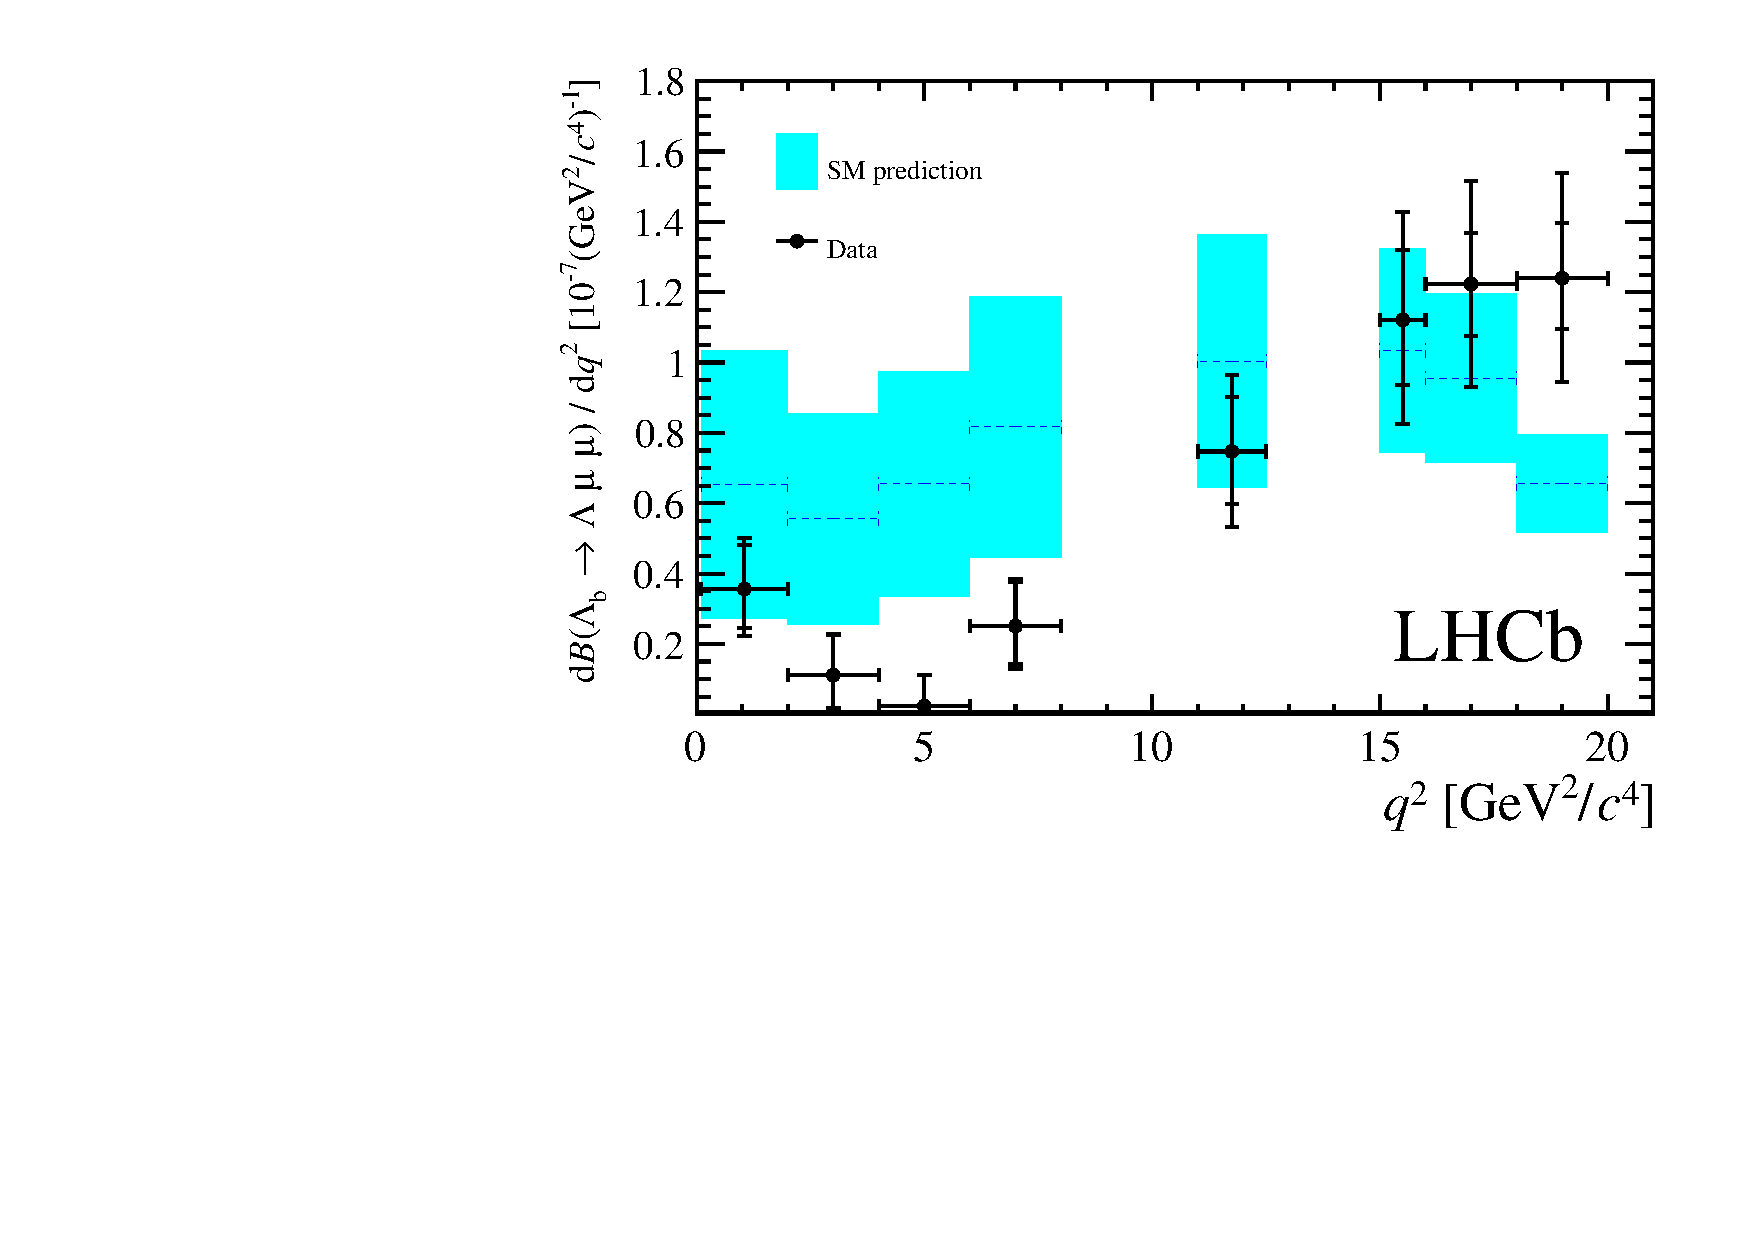
\includegraphics[width=0.8\textwidth]{Lmumu/figs/paper/figure5.pdf}
\caption{Measured \protect\decay{\Lb}{\Lz\mumu} branching
   fraction as a function of \qsq with the predictions of the SM
   \cite{Detmold:2012vy} superimposed.  The inner error bars on data
   points represent the total uncertainty on the relative branching
   fraction (statistical and systematic); the outer error bar also
   includes the uncertainties from the branching fraction of the
   normalisation mode.}  
\label{fig:Lb_absBR}
\end{figure}

\begin{table}[tbph]
\centering
\renewcommand{\arraystretch}{1.2}
\caption{Measured differential branching fraction of
  \decay{\Lb}{\Lz\mumu}, where the uncertainties are statistical, systematic and
 due to the uncertainty on the normalisation mode, \decay{\Lb}{\jpsi\Lz}, respectively.}
\begin{tabular}{ccccccc}
  \qsq interval  [\gevgevcccc] & &\multicolumn{5}{c}{$\deriv \BF(\decay{\Lb}{\Lz\mumu})/\deriv\qsq \cdot 10^{-7} [(\gevgevcccc)^{-1}]$} \\
\hline
0.1 -- 2.0    &    &0.36  &  $^{+\,0.12}_{-\,0.11}$   & $^{+\,0.02}_{-\,0.02}$ & $\pm\,0.07$ \\
2.0 -- 4.0    &    &0.11  &  $^{+\,0.12}_{-\,0.09}$   & $^{+\,0.01}_{-\,0.01}$ & $\pm\,0.02$ \\
4.0 -- 6.0    &    &0.02  &  $^{+\,0.09}_{-\,0.00}$   & $^{+\,0.01}_{-\,0.01}$ & $\pm\,0.01$ \\
6.0 -- 8.0    &    &0.25  &  $^{+\,0.12}_{-\,0.11}$   & $^{+\,0.01}_{-\,0.01}$ & $\pm\,0.05$ \\

11.0 -- 12.5  &    &0.75  &  $^{+\,0.15}_{-\,0.14}$   & $^{+\,0.03}_{-\,0.05}$ & $\pm\,0.15$ \\
15.0 -- 16.0  &    &1.12  &  $^{+\,0.19}_{-\,0.18}$   & $^{+\,0.05}_{-\,0.05}$ & $\pm\,0.23$ \\
16.0 -- 18.0  &    &1.22  &  $^{+\,0.14}_{-\,0.14}$   & $^{+\,0.03}_{-\,0.06}$ & $\pm\,0.25$ \\
18.0 -- 20.0  &    &1.24  &  $^{+\,0.14}_{-\,0.14}$   & $^{+\,0.06}_{-\,0.05}$ & $\pm\,0.26$ \\

\hline
1.1 -- 6.0    &    &0.09  &  $^{+\,0.06}_{-\,0.05}$   & $^{+\,0.01}_{-\,0.01}$ & $\pm\,0.02$ \\
15.0 -- 20.0  &    &1.20  &  $^{+\,0.09}_{-\,0.09}$   & $^{+\,0.02}_{-\,0.04}$ & $\pm\,0.25$ \\
 \end{tabular}
\label{tab:Lb_absBR}
\end{table}





\clearpage
